\section{Zeeman-Effekt}\label{sec:zeeman}
Der Zeeman-Effekt beschreibt die Aufspaltung der Energieniveaus einzelner Zustände 
in einem Magnetfeld. Spin und Bahndrehimpuls bewirken ein magnetisches Moment, auf welches 
ein äußere Magnetfeld wirken kann. Quantenmechanisch kann dies durch den Hamiltonoperator 
beschrieben werden, der die Interaktion mit einem äußeren Feld beschreibt \cite{Sakurai}:
\begin{equation}
    \hat H_\mathrm{int} = -\frac{q}{2m_\mathrm e}\qty(\hat{\vec L} + 2\hat{\vec S})\cdot \vec B.
    \label{eq:zeeman_hamilton}
\end{equation}

In diesem Versuch wird die Aufspaltung an Cadmium beobachtet. Das äußere Elektron sieht 
aufgrund der Wahrscheinlichkeitsverteilung in erster Näherung den Kern mit den inneren 
Schalen effektiv als nur ein Teilchen, womit die Berechnung der Energieniveaus 
äquivalent zum Wasserstoffatom betrachtet werden kann. Da dieses durch eine gerade 
Elektronenzahl keinen Gesamtspin 
besitzt und das Magnetfeld homogen ist, vereinfacht sich \cref{eq:zeeman_hamilton} zu 
\begin{equation*}
    \hat H_\mathrm{int} = \frac{eB}{2m_\mathrm e}\hat{L_z},
\end{equation*}
wobei die Elektronenladung eingesetzt wurde und das Magnetfeld per Konvention in die z-Achse zeigt.
Da bei kugelsymmetrischem Potenzial die z-Komponente des Drehimpulsoperators mit dem restlichen Hamiltonoperator
des Atoms kommutiert, ergibt sich eine Verschiebung des Energieniveaus von
\begin{equation*}
    \Delta E = \frac{e\hbar}{2m_\mathrm e}m_jB \equiv \mu_\mathrm B m_j B
    \label{eq:energy_zeeman}
\end{equation*}

mit dem Bohrschen Magneton \cite{Demtröder:829119}
\begin{equation}
    \mu_B = \SI{9.274015}{\joule\per\tesla}.
    \label{eq:magneton}
\end{equation}
Weil hier elektrische Dipolübergänge betrachtet werden, gilt die Auswahlregel 
$\Delta m = \{\pm 1, 0\}$ \cite{Demtröder:829119}, wobei einer Differenz 
von null linear polarisiertes Licht (im folgenden als $\pi$ bezeichnet) und einer Differenz von $\pm 1$
zirkular polarisiertes Licht ($\sigma^+$ für links zirkular und $\sigma^-$ für rechts zirkular) 
zugeordnet werden kann.
Für $\pi$-Polarisation kann daher keine Energieverschiebung beobachtet werden, für 
$\sigma^\pm$-Polarisation eine Verschiebung von 
\begin{equation}
    \delta E = \pm \mu_\mathrm B B
    \label{eq:normal_zeeman}.
\end{equation}
Unabhängig von der Drehimpulsquantenzahl kann somit beim hier beschriebenen 
normalen Zeeman-Effekt immer nur eine Aufspaltung in drei Linien beobachtet werden,
weshalb die Entartung nur teilweise aufgehoben werden kann.

In \cref{fig:zeeman_übergänge} ist das Übergangsschema für die Übergänge ${}^1D_2\rightarrow {}^1P_1$
des Cadmiumatoms dargestellt. Die Wellenlänge des Übergangs ist $\lambda_0 = \SI{644}{\nano\meter}$
und entspricht rotem Licht. Dieser Übergang wird in diesem Versuch untersucht.

\begin{figure}
    \centering
    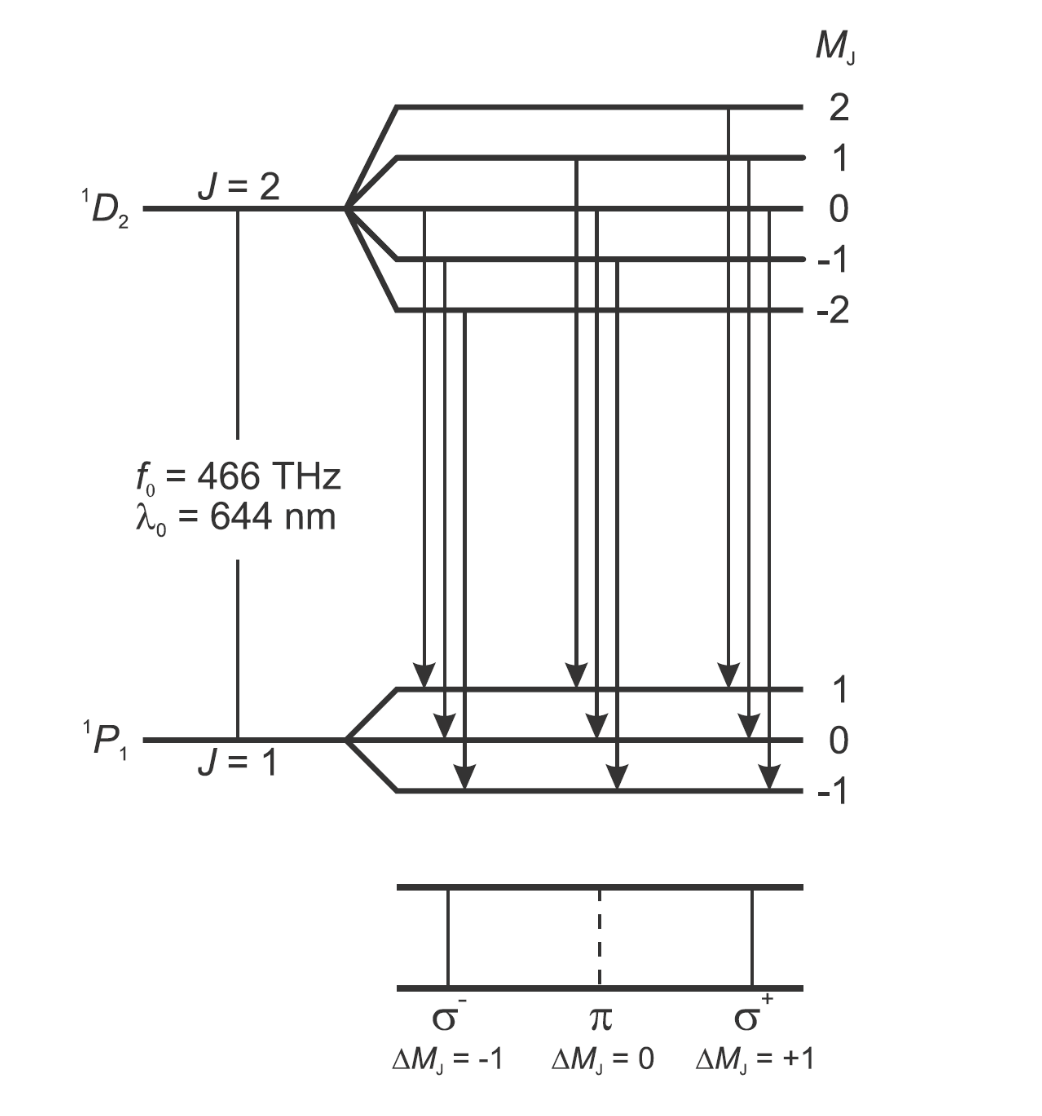
\includegraphics[width=0.6\linewidth]{../figs/zeeman_übergänge}
    \caption{Übergangsschema von Cadmium für die Singulett-Zustände ${}^1D_2\rightarrow {}^1P_1$. 
        Zusehen sind jeweils drei Übergangsgruppen mit je drei Übergängen, die untereinander
        entartet sind, die Entartung zwischen einander jedoch durch den Zeeman-Effekt aufgehoben wird. Darunter 
        ist die durch die Auswahlregeln bestimmte Polarisation des abgestrahlten Lichts aufgetragen. 
        \cite{zeeman_handblatt}}
    \label{fig:zeeman_übergänge}
\end{figure}

\subsection{Versuchsaufbau}
Der Aufbau zur Untersuchung des Zeeman-Effekts ist in \cref{fig:zeeman_aufbau} skizziert. Eine 
Cadmiumlampe wird zwischen ein Magnetfeld festgehalten, welches durch zwei in Reihe 
geschalteten stromdurchflossenen Spulen erzeugt wird. Die Spulen können 
um die vertikale Achse gedreht werden, um die Richtung 
des Magnetfeldes in Bezug zur Beobachtungsrichtung verändern zu können. 
Das Licht der Lampe wird mit einer Kondensorlinse 
$f=\SI{150}{\mm}$ kollimiert mit leichter Konvergenz, um nachher am Etalon verschieden Einfallswinkel zu 
erzeugen. 

Das eingebaute Fabry-P\'erot-Etalon ist eine planparallele Glasschicht, welche 
beidseitig mit teildurchlässigen Spiegeln beschichtet ist. Durch ständige Reflexion innerhalb der Glasschicht
wird ein Strahlenbündel erzeugt, welches durch Gangunterschiede untereinander interferiert. 
Das hier benutzte Etalon hat einen Brechungsindex von $n=1.457$ und einem Reflexionsgrad $R=0.85$.
Mit einer weiteren Sammellinse $f=\SI{150}{\mm}$ wird das Licht am Okular scharf abgebildet, an 
dem durch die entstandene Interferenz konzentrische Ringe Beobachter sein können. Davor wird mit einem 
Interferenzfilter das rote Licht bei $\SI{644}{\nm}$ gefiltert.

\begin{figure}[h]
    \centering
    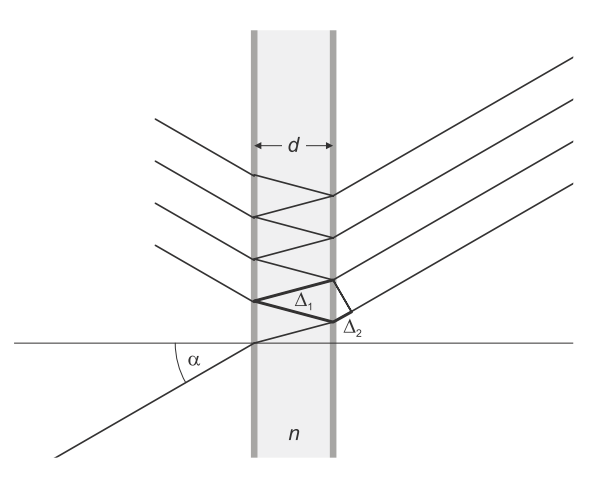
\includegraphics[width=0.6\linewidth]{../figs/etalon}
    \caption{Funktionsweise eines Fabry-P\'erot-Etalon. $\alpha$ bezeichnet den Einfallswinkel 
        eines Lichtstrahls in den Etalon mit Dicke $d$ bei Brechungsindex $n$.
        $\Delta_1$ und $\Delta_2$ bezeichnen die Gangunterschiede, die zur Interferenz zweier 
        transmittierter Strahlen führen.
        \cite{zeeman_handblatt}}
    \label{fig:etalon}
\end{figure}

\begin{figure}[h]
    \centering
    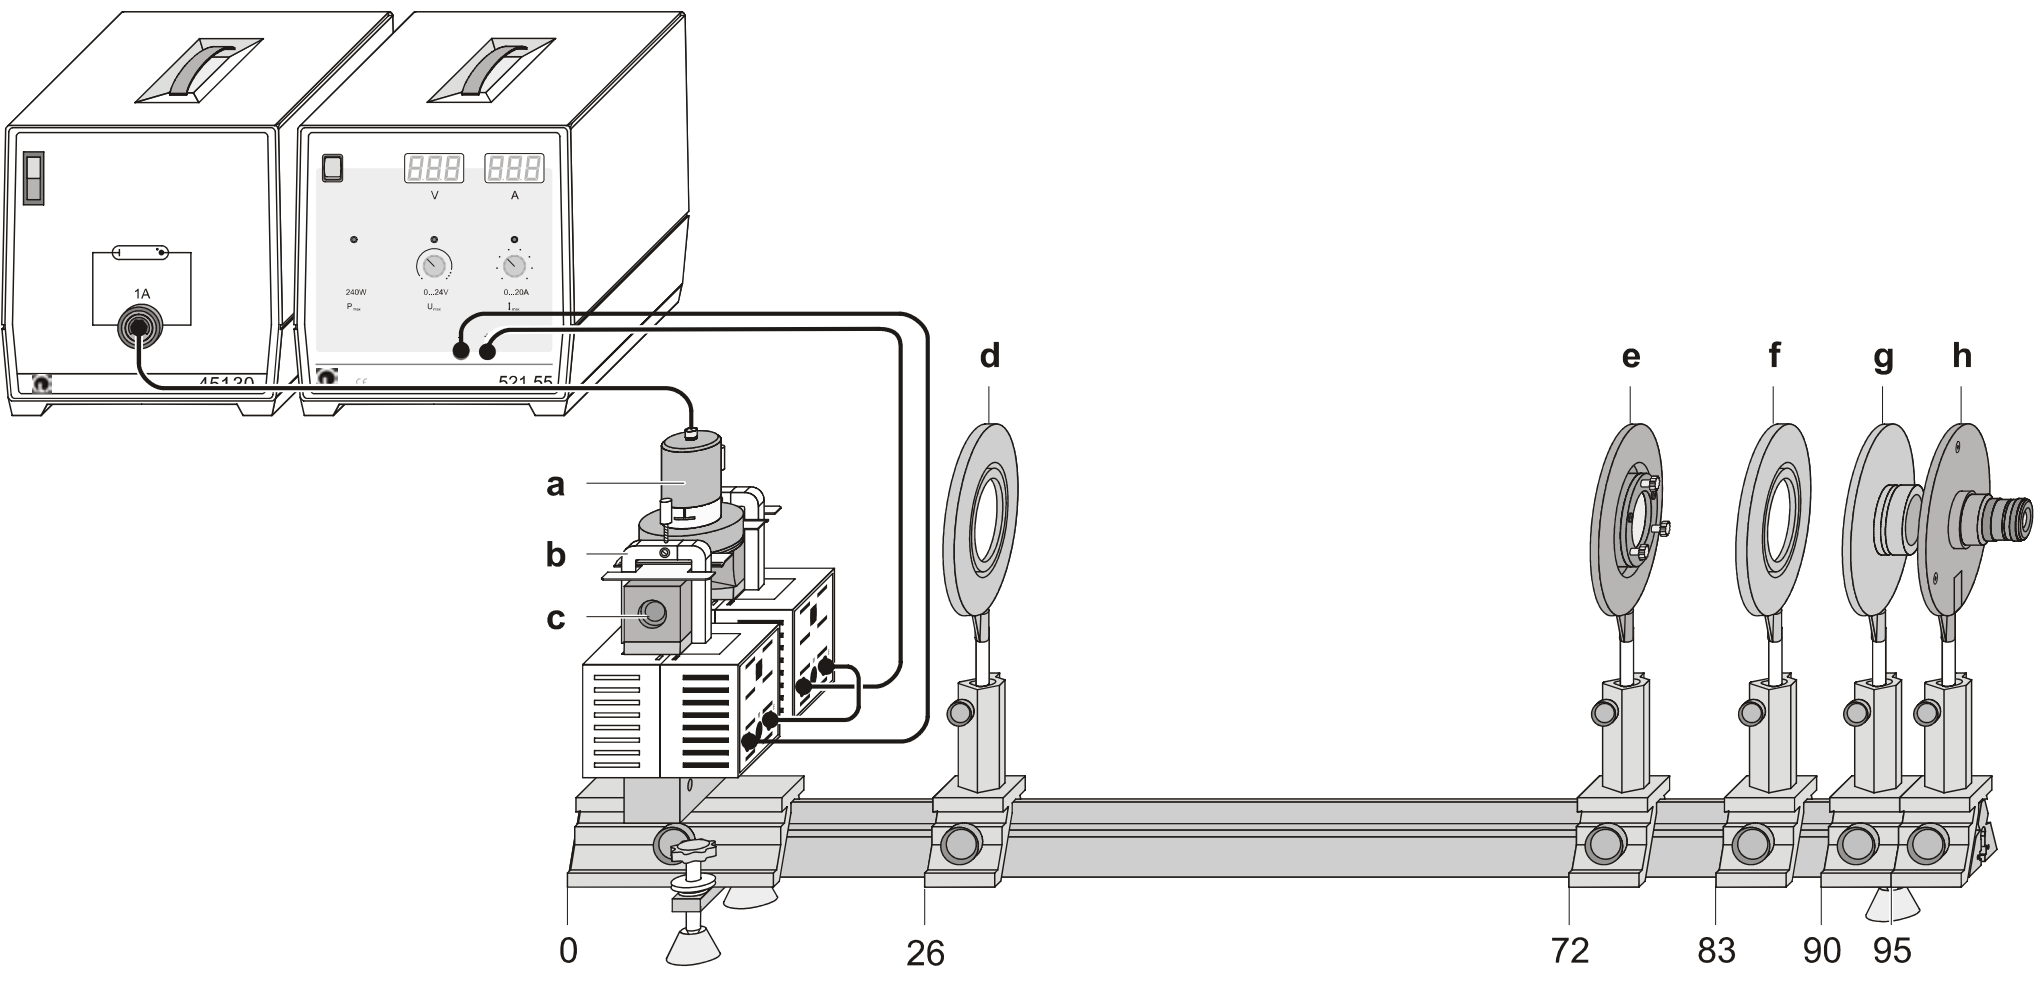
\includegraphics[width=0.7\linewidth]{../figs/zeeman_aufbau}
    \caption{Aufbau zur Messung des Zeeman-Effekts. \abf a zeigt die Cadmiumlampe mit Klammern
        \abf b und Polschuhe \abf c. \abf d zeigt die Kondensorlinse, \abf e das Etalon, \abf f 
        die Abbildungslinse, \abf g das Interferenzfilter und \abf h das Okular mit Strichskala. 
        \cite{zeeman_handblatt}}
    \label{fig:zeeman_aufbau}
\end{figure}

\subsection{Untersuchung der Transversal- und Longitudinalkonfiguration}\label{sec:zeeman_quantitativ}
Durch das Drehen der Spulen lässt sich die Polarisation der emittierten Strahlung 
untersuchen. Hierbei werden zwei Konfigurationsmöglichkeiten gesondert betrachtet.
Klassisch lässt sich die Polarisations- und Strahlrichtung der Übergangsstrahlung 
mit dem Lorentz-Modell beschreiben, wo eine Schwingungsgleichung mit der Lorentzkraft als 
treibende Kraft angesehen wird. Dabei sind $\pi$- und $\sigma^\pm$-Strahlung die Eigenmodi 
der Lösung. Diese sind in \cref{fig:zeeman_polarisation} skizziert. Zu sehen ist hierbei, 
dass sich jede Lösung als schwingender Dipol interpretieren lässt, wobei für $\sigma^\pm$ 
zwei senkrecht zueinander stehenden Dipole mit einer $\SI{90}{\degree}$-Phasenbeziehung 
betrachtet werden.

Da Dipole nicht in Bewegungsrichtung abstrahlen, kann in longitudinaler 
Beobachtungsrichtung (parallel zum Magnetfeld) nur die zirkular polarisierte $\sigma^\pm$-Strahlung
beobachtet werden. Bei transversaler Konfiguration sind alle drei Modi sichtbar mit dem 
Unterschied, dass $\sigma^\pm$ hier linear polarisiert ist und räumlich um $\SI{90}{\degree}$
zur $\pi$-Polarisation gedreht.

\subsubsection{Transversalkonfiguration}
In Transversalrichtung können $\sigma^\pm$- sowie $\pi$-Strahlung beobachtet werden, wobei 
diese Modi linear polarisiert sind und senkrecht zueinander stehen. Mit einem Polarisationsfilter 
lässt sich somit $\pi$ und $\sigma$ voneinander trennen, $\sigma^+$ und $\sigma^-$ sind jedoch nicht 
unterscheidbar voneinander. Vor das Etalon wird der Polarisationsfilter befestigt und 
beim Einschalten des Magnetfeldes das Bild beobachtet. Die optische Achse 
des Filters steht auf $\SI{0}{\degree}$, wenn Diese senkrecht zur optischen Bank
steht. Erwartet wird das Verschwinden der inneren Ringe bei einer Filterausrichtung von 
\SI{0}{\degree}, da in diesem Falle die optische Achse des Filters senkrecht zum B-Feld und damit 
zur Polarisationsachse des $\pi$-Lichts steht. Damit ist das Verschwinden der äußeren Ringe 
bei \SI{90}{\degree} zu erwarten.

In \cref{fig:transversal_konfiguration} sind die Interferenzringe abgebildet. Durch das Anlegen
eines Magnetfeldes wurde die Aufspaltung der Ringe in einen hellen mittleren 
Ring und zwei leicht dunklere daneben deutlich. Aufgrund des Auflösungsvermögens und möglicherweise 
einer Überbelichtung konnten die Details des Bildes auf der Aufnahme nicht kenntlich
gemacht werden. Bei einer Polarisationsfiltereinstellung von \SI{0}{\degree} verschwinden
die inneren Ringen, bei \SI{90}{\degree} die Äußeren. Dies entspricht dem erwarteten Verhalten, 
weshalb daraus geschlossen werden kann, dass das Licht der äußeren Ringe senkrecht zum 
B-Feld polarisiert ist und das Licht der inneren Ringe parallel dazu.

\begin{figure}[h]
    \centering
    \begin{subfigure}{0.45\linewidth}
        \centering
        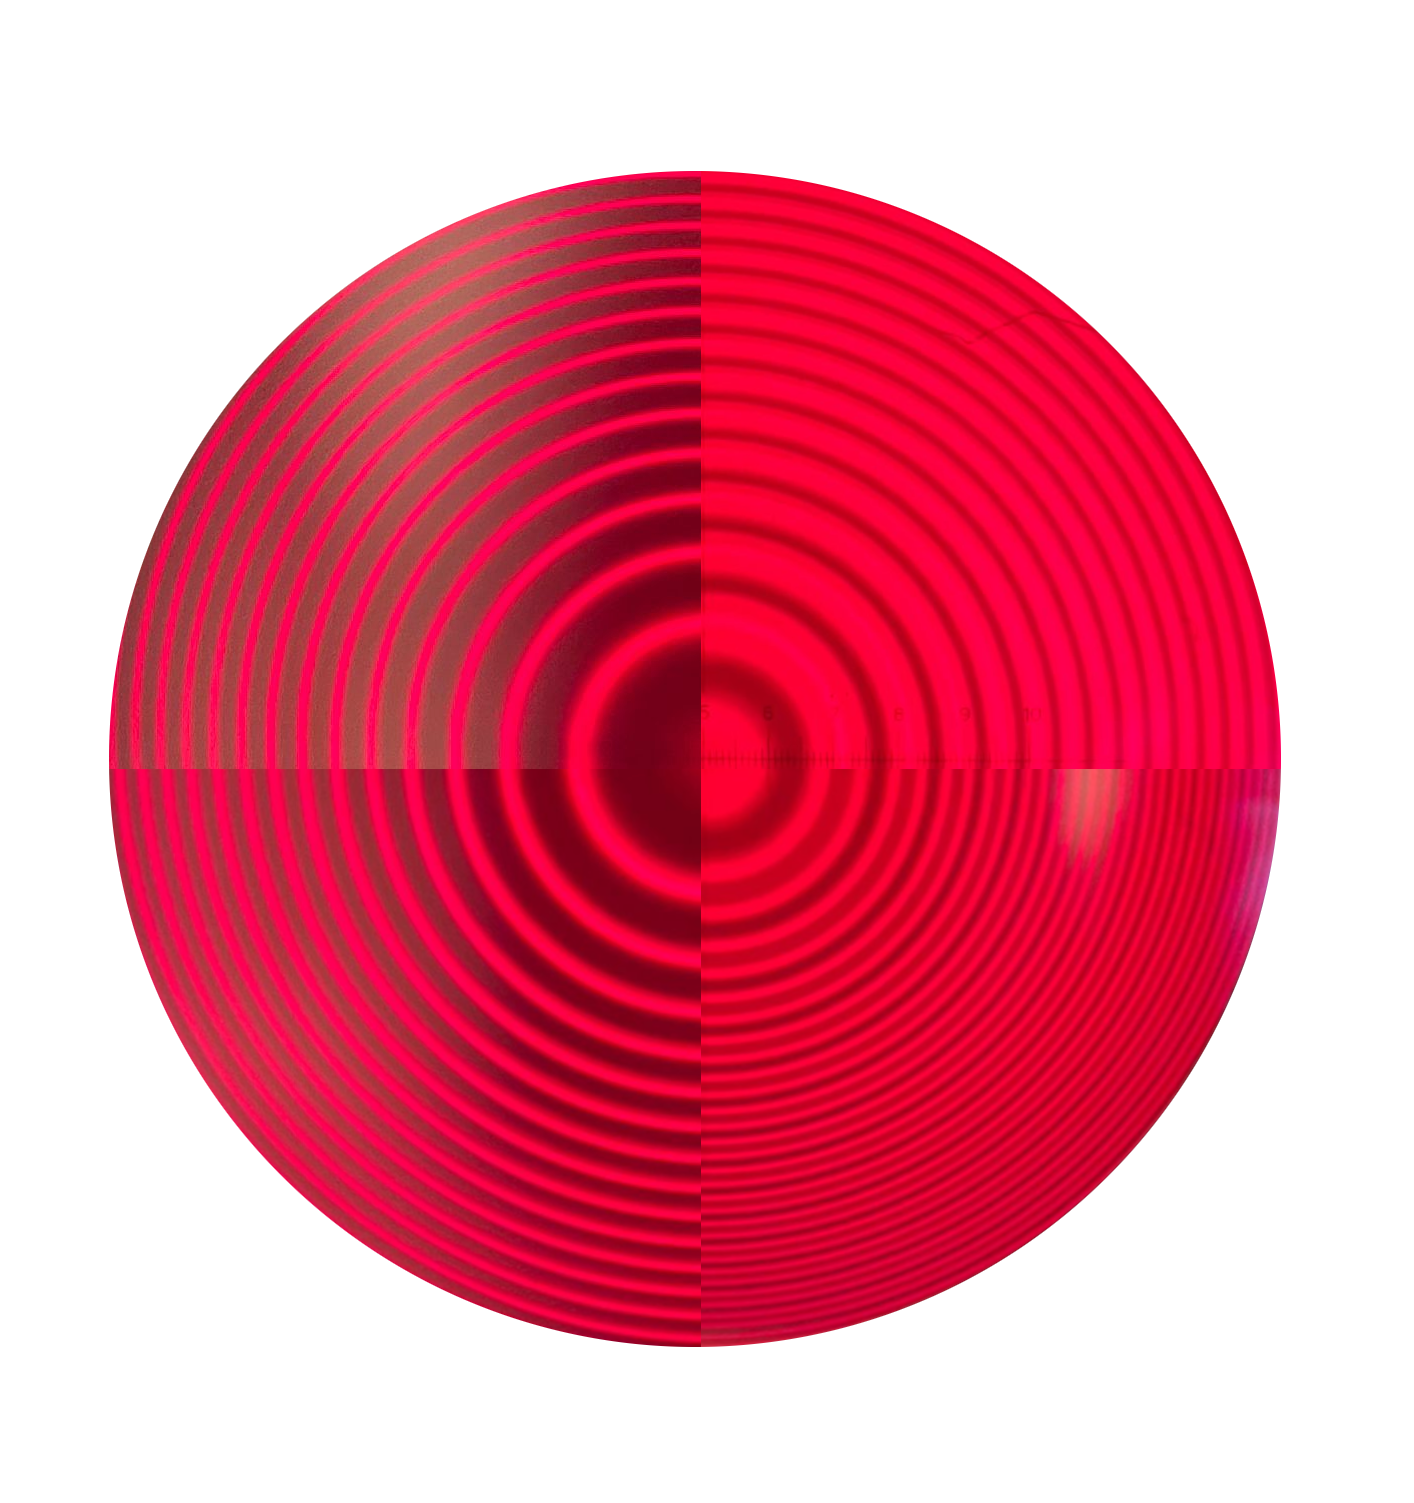
\includegraphics[width=\linewidth]{../figs/transversal_konfig}
        \caption{Transversal Konfiguration: links oben ohne B-Feld, rechts oben mit B-Feld,
            rechts unten mit Filter auf $\SI{0}{\degree}$, links unten mit Filter auf $\SI{90}{\degree}$.}
        \label{fig:transversal_konfiguration}
    \end{subfigure}
    \hspace{.5cm}
    \begin{subfigure}{0.45\linewidth}
        \centering
        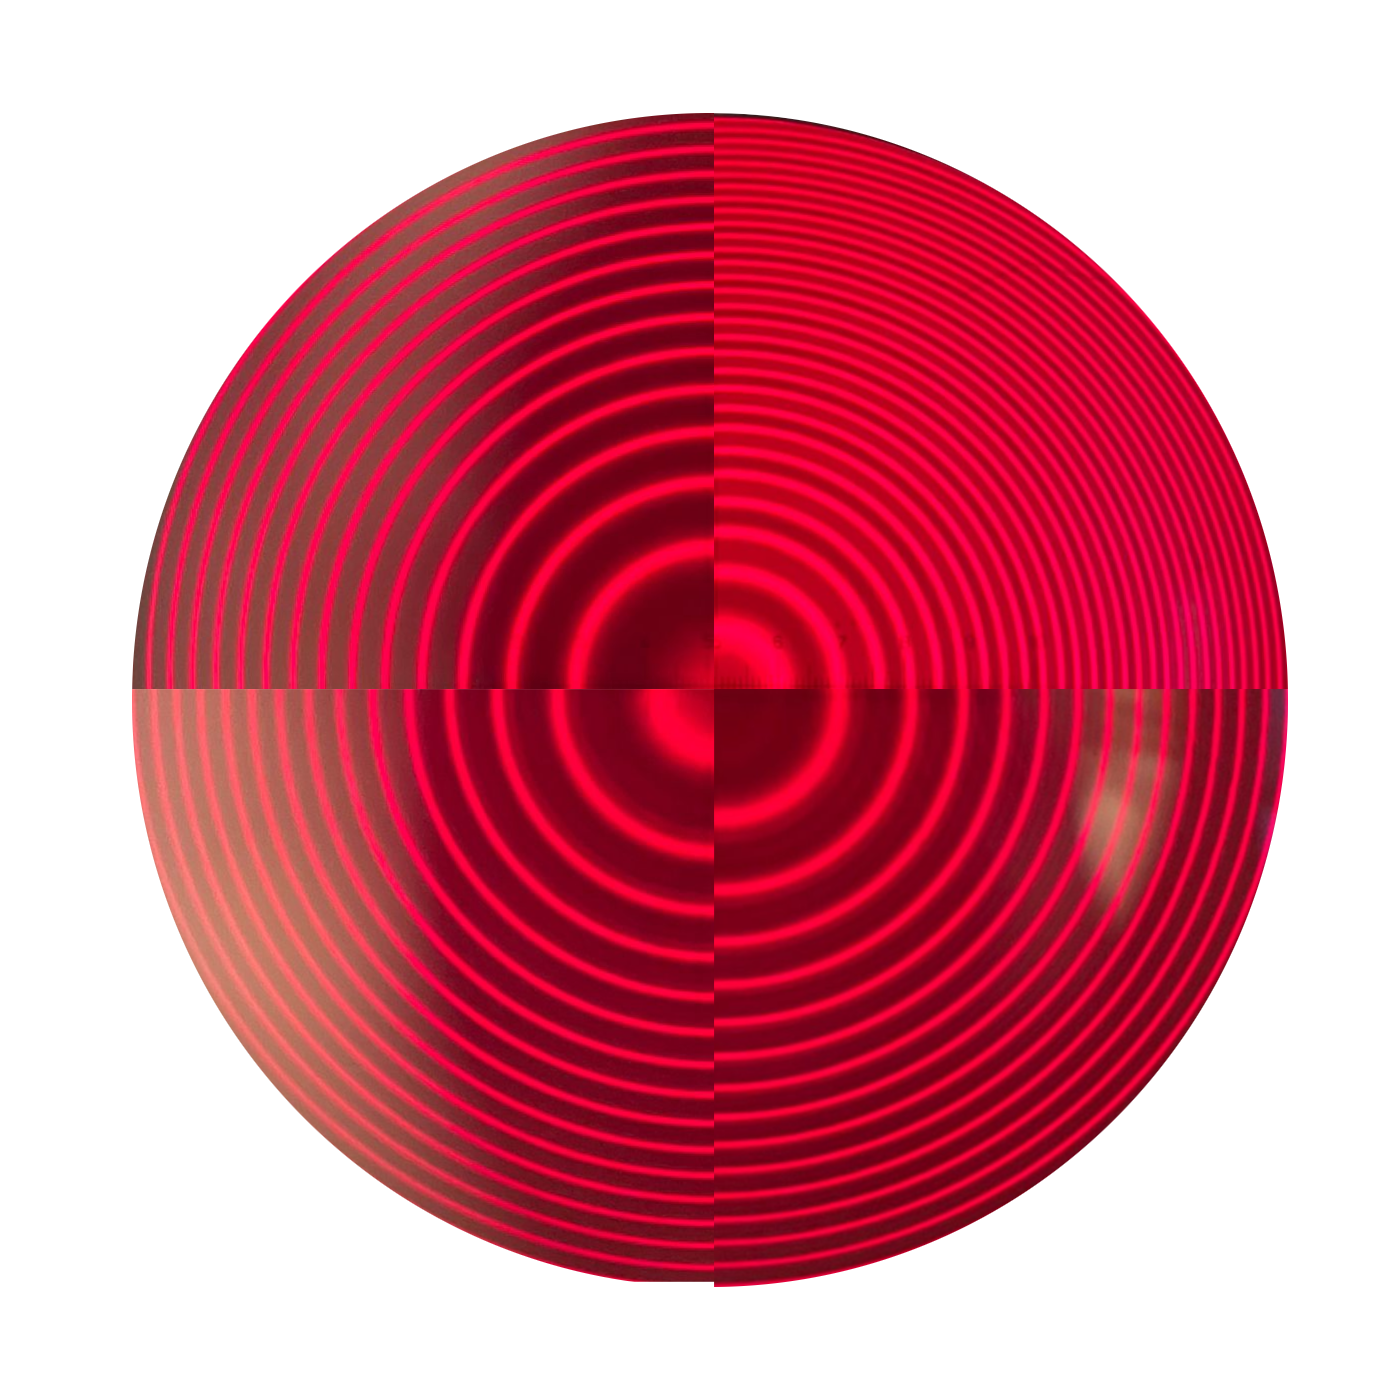
\includegraphics[width=\linewidth]{../figs/longitudinal_konfig}
        \caption{Longitudinal Konfiguration: links oben ohne B-Feld, rechts oben mit B-Feld, 
        rechts unten mit Filter auf $\SI{+45}{\degree}$, links unten mit Filter auf $\SI{-45}{\degree}$. }
        \label{fig:longitudinal_konfiguration}
    \end{subfigure}
    \caption{Aufnahmen der Etalon Interferenzringe bei unterschiedlichen Aufbauten.}
\end{figure}


\subsubsection{Longitudinalkonfiguration}
In longitudinaler Ausrichtung kann nur das $\sigma^\pm$-Licht beobachtet werden. Um zu zeigen, 
dass beide Wellen zirkular und entgegengesetzt polarisiert sind, wird vor dem Polarisationsfilter 
eine $\lambda/4$-Wellenplatte befestigt, welche die Phase des elektrischen Feldes parallel 
zur optischen Achse um eine viertel Wellenlänge verschiebt und somit zirkulares Licht 
linear polarisieren kann. Per Definition entsprechen $\sigma^\pm$ die komplexen Vektoren des 
elektrischen Feldes 
$\vb E_\mathrm{\sigma^\mp} \propto \vb e_x \mp i\vb e_y$. Ohne Beschränkung der Allgemeinheit wird die optische Achse 
der Wellenplatte auf die y-Achse gesetzt. Bei einer Verzögerung wird die y-Komponente 
um den Faktor $\e^{\pm i\pi /2} = \pm i$ verschoben, womit sich eine Polarisation von 
$\vb E_\mathrm{\sigma^\mp}\propto \vb e_x \pm \vb e_y$ ergibt. Somit ist $\sigma^-$ 
bei einer Ausrichtung des Filters bei \SI{45}{\degree} sichtbar, während $\sigma^+$ Licht 
bei \SI{-45}{\degree} sichtbar wird. 

In \cref{fig:longitudinal_konfiguration} ist die Longitudinalkonfiguration gezeigt. Es ist zu erkennen,
das sich diesmal beim Anlegen eines Magnetfeldes die Linie in nur zwei symmetrisch verteilte Linien 
aufspaltet. Nach Durchgang einer Verzögerungsplatte und einer Filtereinstellung von $\pm\SI{45}{\degree}$
verschwindet wie erwartet jeweils einer der zwei Ringe. Aufgrund der oberen Überlegung 
lässt sich damit der innere Ring $\sigma^-$-Licht zuweisen und $\sigma^+$-Licht dem äußeren Ring.
Auf die Relation, dass $\sigma^-$ kleinere Winkel und $\sigma^+$ größere Winkel zuzuordnen sind, wird 
bei der Bestimmung des Bohr Magnetons weiter eingegangen.


\begin{figure}[htb]
    \centering
    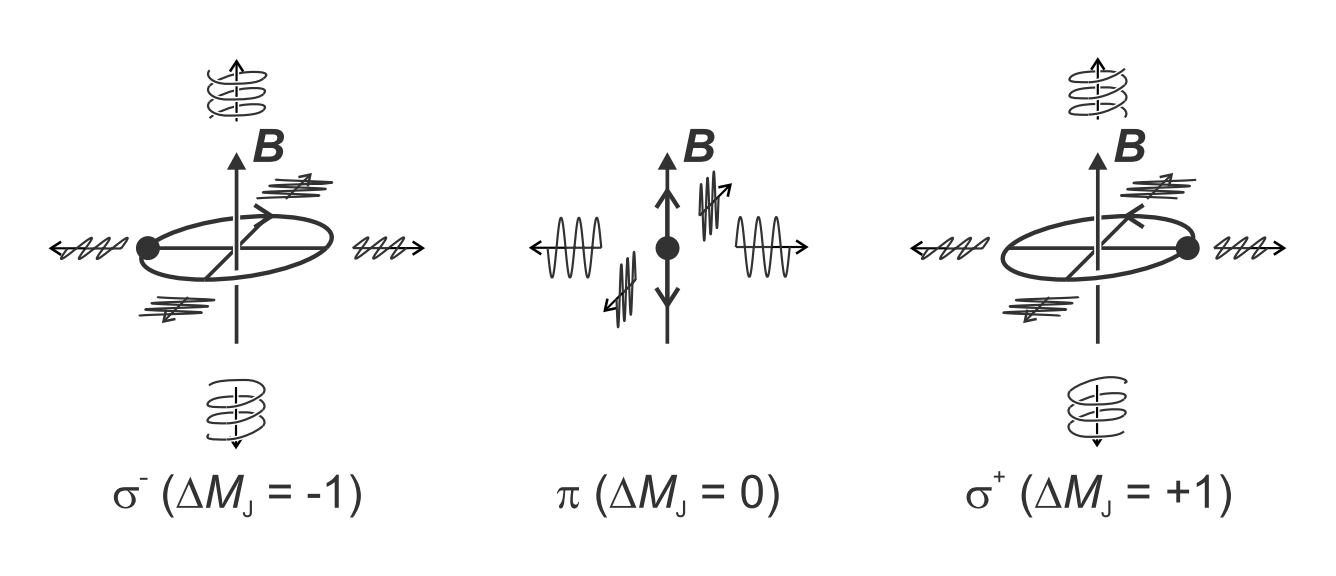
\includegraphics[width=0.6\linewidth]{../figs/zeeman_polarisation}
    \caption{Polarisation der verschiedenen Übergänge. $\pi$-Strahlung ist nur in transversaler 
    Richtung beobachtbar, $\sigma^\pm$-Strahlung in transversaler und in longitudinaler 
    Richtung. \cite{zeeman_handblatt}}
    \label{fig:zeeman_polarisation}
\end{figure}

\subsection{Bestimmung des Bohrschen Magnetons}\label{sec:magneton}
Zur Bestimmung des Bohrschen Magnetons wird die Aufspaltung der Linien 
in Transversalkonfiguration mit einer CCD-Kamera gemessen. Diese Messung wird 
bei unterschiedlichen Spulenströmen 40-mal durchgeführt und der Mittelwert 
gespeichert für genauere Ergebnisse. Mit einer Hall-Sonde wird 
zur Kalibration das Magnetfeld in Abhängigkeit des Stroms vor und nach der Durchführung
einer Messung vorgenommen. Durch das Erhitzen der Spulen wird erwartet, dass sich 
die Kalibrationskurve mit der Zeit ändert. Durch zwei Messungen kann damit der Fehler des 
Magnetfeldes bestimmt werden.

Untersucht wird hierbei ein einzelnes Interferenzmaximum nahe des Ringzentrums. Dieses wird 
beim Anlegen eines Magnetfeldes in drei Maxima aufgespalten. An die gemessenen Kurven 
werden drei Gauss-Kurven mit einem linearen Offset angepasst. Die Anpassfunktion kann somit beschrieben werden 
mit 
\begin{equation*}
    f(x, \vec x, \vec \sigma, \vec A, m, n) = \sum_{i=1}^3 \frac{A_i}{\sqrt{2\pi}\sigma_i}
        \exp\qty(-\frac{(x-x_i)^2}{2\sigma_i^2}) +mx + n.
\end{equation*}

Das Programm zur Messung der Einstrahlintensitäten gibt keine dazugehörigen Unsicherheiten an.
Aus diesem Grund müssen diese rekonstruiert werden. Die CCD-Kamera misst Photonen, wodurch 
die Messung pro Pixel als Poisson-verteilt angesehen werden kann mit dazugehörigem Poisson-Fehler \\
$\Delta N = \sqrt{N}$. Die Umrechnung der Zählereignisse in eine Intensität (in Prozent) ist unbekannt, 
weshalb der Fehler mit einem unbekannten Faktor skaliert wird. Für die Anpassungskurve 
ist dieser jedoch irrelevant, da nur der relative Fehler der einzelnen Messpunkte von Bedeutung ist. 
Der Skalierungsfaktor ist daher nicht nötig. Da jedoch nur die relativen Fehler bekannt sind, verliert 
die Berechnung einer Anpassungsgüte, wie dem reduzierten Chi-Quadrat \cite{wiki:reduced_chi_square},
seine Bedeutung, weshalb eine quantitative Bewertung der Anpassungen nicht durchgeführt werden kann.

\begin{figure}
    \centering
    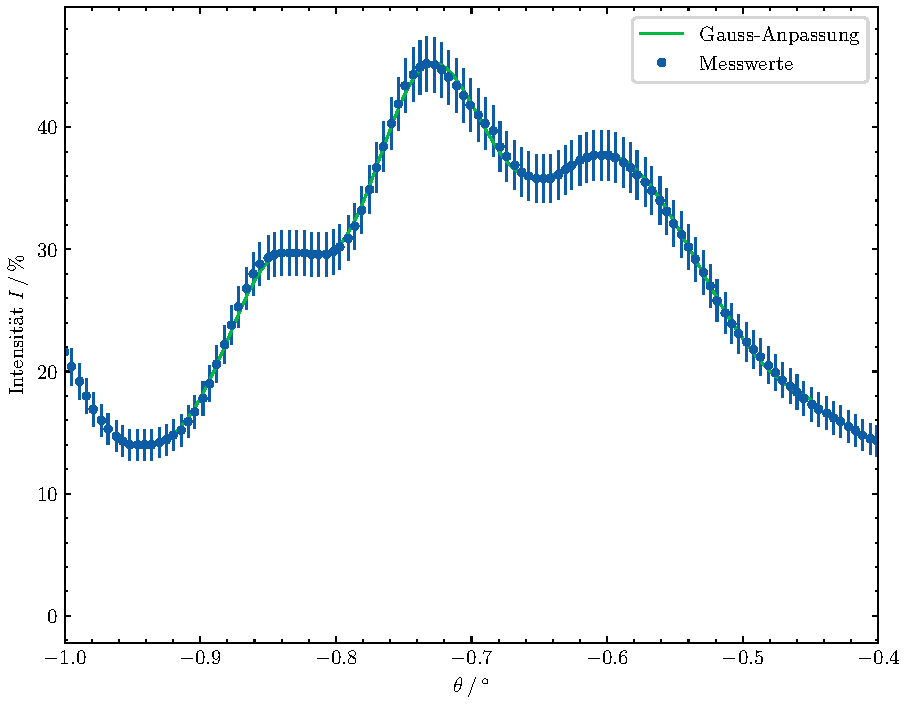
\includegraphics[width=.6\linewidth]{../figs/gauss_i7.9.pdf}
    \caption{Aufspaltung der Maxima bei einem Strom von \SI{7.9}{\ampere}.}
    \label{fig:gauss_i79}
\end{figure}

Eine Anpassungskurve ist beispielhaft in \cref{fig:gauss_i79} gezeigt. Visuell
kann die Anpassung als äußerst erfolgreich angesehen werden. Weitere Diagramme 
sind im \cref{sec:anhang} zu finden.


Die Mittelwerte und Standardabweichungen der Gauß-Kurven sind tabellarisch in \cref{tab:gauss_zeeman_maxima_and_std}
dargestellt. Es fällt auch, dass das mittlere Maximum nicht immer am gleichen Winkel vorzufinden ist. Daraus lässt sich 
schließen, dass während der Messung der Mittelpunkt der Ringe stets in einem kleinen Bereich geschwankt 
ist. Der daraus resultieren Fehler wird für kleine Winkel 
jedoch nur linear mit der Verschiebung ansteigen und im Vergleich zu anderen Fehlern gering sein.
Mit \cref{fig:etalon} lässt sich für die Maxima die Bedingung 
\begin{equation}
    \lambda = \frac{2d}{m}\sqrt{n^2-\sin^2\alpha}, \qquad 
    \Delta\lambda \approx \frac{2d}{m}\frac{\alpha \Delta\alpha}{\sqrt{n^2 - \alpha^2}}
    \label{eq:etalon_gleichung}
\end{equation}
mit der Beugungsordnung $m$ herleiten. Für die Unsicherheit wurde die Kleinwinkelnäherung benutzt, was 
hier keinen Unterschied machen sollte, da diese sowieso auf die erste oder zweite signifikante Stelle
aufgerundet werden.
Mit \cref{eq:etalon_gleichung} und dem mittleren Maximum bei bekannter Wellenlänge von \SI{644}{\nm}
lässt sich die Beugungsordnung bestimmen. Diese lag beim untersuchten Maximum bei 
$m = \num{18104}$.

\begin{table}[htbp]
   \centering
\caption{Maxima und Standardabweichungen der Gauss-Anpassungen}
\begin{tabular}{c c c c c c c}
\hline$I / \unit{\ampere}$ & $x_\mathrm{links} / \unit{\degree}$ & $x_\mathrm{mitte} / \unit{\degree}$ & $x_\mathrm{rechts} / \unit{\degree}$ & $\sigma_\mathrm{links} / \unit{\degree}$ & $\sigma_\mathrm{mitte} / \unit{\degree}$ & $\sigma_\mathrm{rechts} / \unit{\degree}$ \\ 
\hline
$\num{4.7}$ & $\num{-0.8253\pm 0.0013}$ & $\num{-0.7481\pm 0.0011}$ & $\num{-0.6590\pm 0.0018}$ & $\num{0.0292\pm 0.0009}$ & $\num{0.0337\pm 0.0012}$ & $\num{0.076\pm 0.003}$ \\
$\num{5.2}$ & $\num{-0.8288\pm 0.0015}$ & $\num{-0.7438\pm 0.0009}$ & $\num{-0.6394\pm 0.0017}$ & $\num{0.0306\pm 0.0012}$ & $\num{0.0384\pm 0.0014}$ & $\num{0.065\pm 0.003}$ \\
$\num{5.7}$ & $\num{-0.8392\pm 0.0009}$ & $\num{-0.7518\pm 0.0007}$ & $\num{-0.6443\pm 0.0009}$ & $\num{0.033\pm 0.001}$ & $\num{0.0375\pm 0.0008}$ & $\num{0.0689\pm 0.0014}$ \\
$\num{6.0}$ & $\num{-0.839\pm 0.003}$ & $\num{-0.750\pm 0.002}$ & $\num{-0.643\pm 0.003}$ & $\num{0.036\pm 0.004}$ & $\num{0.036\pm 0.002}$ & $\num{0.071\pm 0.005}$ \\
$\num{6.3}$ & $\num{-0.8455\pm 0.0009}$ & $\num{-0.7491\pm 0.0006}$ & $\num{-0.631\pm 0.001}$ & $\num{0.0339\pm 0.0012}$ & $\num{0.0411\pm 0.0008}$ & $\num{0.0642\pm 0.0015}$ \\
$\num{6.7}$ & $\num{-0.8417\pm 0.0009}$ & $\num{-0.7398\pm 0.0007}$ & $\num{-0.617\pm 0.001}$ & $\num{0.0338\pm 0.0011}$ & $\num{0.0428\pm 0.0009}$ & $\num{0.0605\pm 0.0018}$ \\
$\num{7.0}$ & $\num{-0.846\pm 0.003}$ & $\num{-0.742\pm 0.003}$ & $\num{-0.621\pm 0.004}$ & $\num{0.038\pm 0.006}$ & $\num{0.042\pm 0.003}$ & $\num{0.059\pm 0.006}$ \\
$\num{7.3}$ & $\num{-0.850\pm 0.001}$ & $\num{-0.7421\pm 0.0008}$ & $\num{-0.6150\pm 0.0012}$ & $\num{0.0358\pm 0.0017}$ & $\num{0.0443\pm 0.0011}$ & $\num{0.059\pm 0.002}$ \\
$\num{7.8}$ & $\num{-0.8489\pm 0.0013}$ & $\num{-0.738\pm 0.001}$ & $\num{-0.6050\pm 0.0015}$ & $\num{0.036\pm 0.003}$ & $\num{0.0452\pm 0.0013}$ & $\num{0.061\pm 0.003}$ \\
$\num{7.9}$ & $\num{-0.8451\pm 0.0012}$ & $\num{-0.735\pm 0.001}$ & $\num{-0.5992\pm 0.0014}$ & $\num{0.0355\pm 0.0017}$ & $\num{0.0444\pm 0.0012}$ & $\num{0.0646\pm 0.0019}$ \\
\hline\end{tabular}
\label{tab:gauss_zeeman_maxima_and_std}
\end{table}

Im Folgenden wird die Wellenlängendifferenz eines äußeren und dem mittleren Maximum als 
\\$\delta\lambda = \lambda_{\sigma^\pm} - \lambda_\pi$ definiert. Damit ist die 
Energieverschiebung gegeben mit 
\begin{equation}
    \delta E = hc\qty(\frac{1}{\lambda_{\sigma^\pm}} - \frac{1}{\lambda_0})
        \equiv -E_0\frac{\delta\lambda}{\lambda_0+\delta\lambda}, \qquad
        \Delta(\delta E) = \delta E \frac{\Delta(\delta\lambda)}{\delta\lambda},
        \label{eq:energieverschiebung}
\end{equation}
wobei für den Fehler $\lambda_0\gg\delta\lambda$ angenommen wurde.
Aufgrund von \cref{eq:etalon_gleichung} lässt sich sagen, das im betrachteten Bereich 
die Wellenlänge steigen muss bei kleineren Winkeln. Da eine höhere Wellenlänge zu kleineren 
Energien führt, führen kleinere Winkel zu kleineren Energien. Damit also 
$\delta E_{\sigma^\pm} = \pm \mu_\mathrm B B$ ist, muss $|\alpha_{\sigma^+}| > |\alpha_0|$
und $\abs{\alpha_{\sigma^-}} < \abs{\alpha_0}$ sein. Aus diesem Grund 
lässt sich das rechte Maximum (innerer Ring) $\sigma^-$ und das linke Minimum 
(äußerer Ring) $\sigma^+$ zuweisen, da negative Winkel betrachtet wurden. Dies stimmt mit 
den Überlegungen in \cref{sec:zeeman_quantitativ} überein.

\begin{figure}[htb]
    \centering
    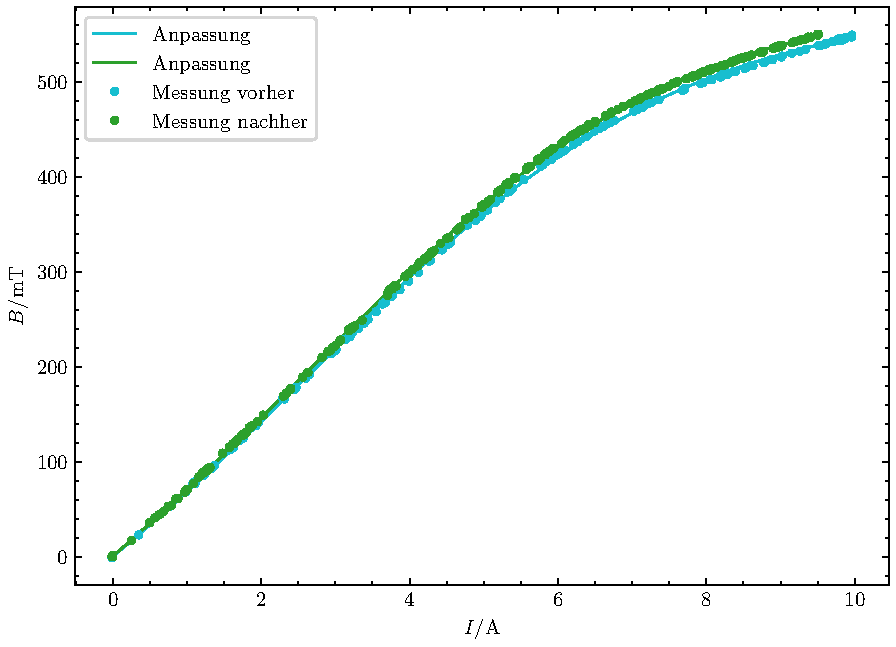
\includegraphics[width=.6\linewidth]{../figs/BFeld-Kalibrationskurve}
    \caption{Magnetfeldkalibration}
    \label{fig:bfield_kalibration}
\end{figure}

Um das Magneton zu bestimmen, muss zusätzlich die Magnetfeldkalibration durchgeführt werden, da 
bei der Messung nur die Spulenströme gemessen wurden. Auch hier sind die Fehler nicht bekannt. 
Da aber die Messung automatisch von dem Programm vorgenommen wurde und manuell der Spulenstrom 
langsam hochgedreht wurde, befinden sich in den Messdaten Bereiche, wo das Magnetfeld
mehrmals beim gleichen Strom gemessen wurde. Die Standardabweichung dieses Bereiches 
wird als Unsicherheit für die Messung genutzt.


Für die Anpassung wird an die Messdaten der Hall Sonde vor und nach der Messung der Interferenzringe 
die Funktion 
\begin{equation*}
    B(I) = \alpha + \frac{\beta}{(\gamma + \e^{-\delta I})^\varepsilon}
\end{equation*}
angepasst. In \cref{fig:kalibration_tabelle} sind die angepassten Parameter tabelliert 
und in \cref{fig:bfield_kalibration} die Anpassungsfunktionen mit den Messwerten 
grafisch dargestellt. Da für beide Kalibrationskurven das resultierende $\chi^2$
klein ist und diese visuell betrachtet nicht von den Messdaten unterscheidbar sind,
kann die Kalibration für die weitere Auswertung genutzt werden. Es kann angenommen werden,
das während der Messung sich das tatsächliche Magnetfeld zwischen den beiden Kalibrationskurven
befand. Aus diesem Grund wird für kommende Rechnungen der Mittelwert beider 
Kurven verwendet mit 
\[B(I) = \frac{B_\mathrm{vor}(I) + B_\mathrm{nach}(I)}{2}, 
\qquad \Delta B(I) = \abs{\frac{B_\mathrm{vor}(I) - B_\mathrm{nach}(I)}{2}}.\]

\begin{table}[h]
   \centering
\caption{Anpassparameter der Magnetfeldkalibration}
\begin{tabular}{c c c c c c c}
\hline Magnetfeldmessung & $\alpha / \unit{\milli\tesla}$ & $\beta / \unit{\milli\tesla}$ & $\gamma$ & $\delta$ & $\epsilon$ & $\chi^2$ \\ 
\hline
vorher & $\num{-1140\pm 120}$ & $\num{1150\pm 120}$ & $\num{0.022\pm 0.003}$ & $\num{0.621\pm 0.014}$ & $\num{0.092\pm 0.011}$ & $\num{7.15}$ \\
nachher & $\num{-1100\pm 70}$ & $\num{1100\pm 70}$ & $\num{0.0097\pm 0.0012}$ & $\num{0.748\pm 0.015}$ & $\num{0.074\pm 0.006}$ & $\num{1.89}$ \\
\hline\end{tabular}
\label{fig:kalibration_tabelle}
\end{table}

\begin{figure}[htb]
    \centering
    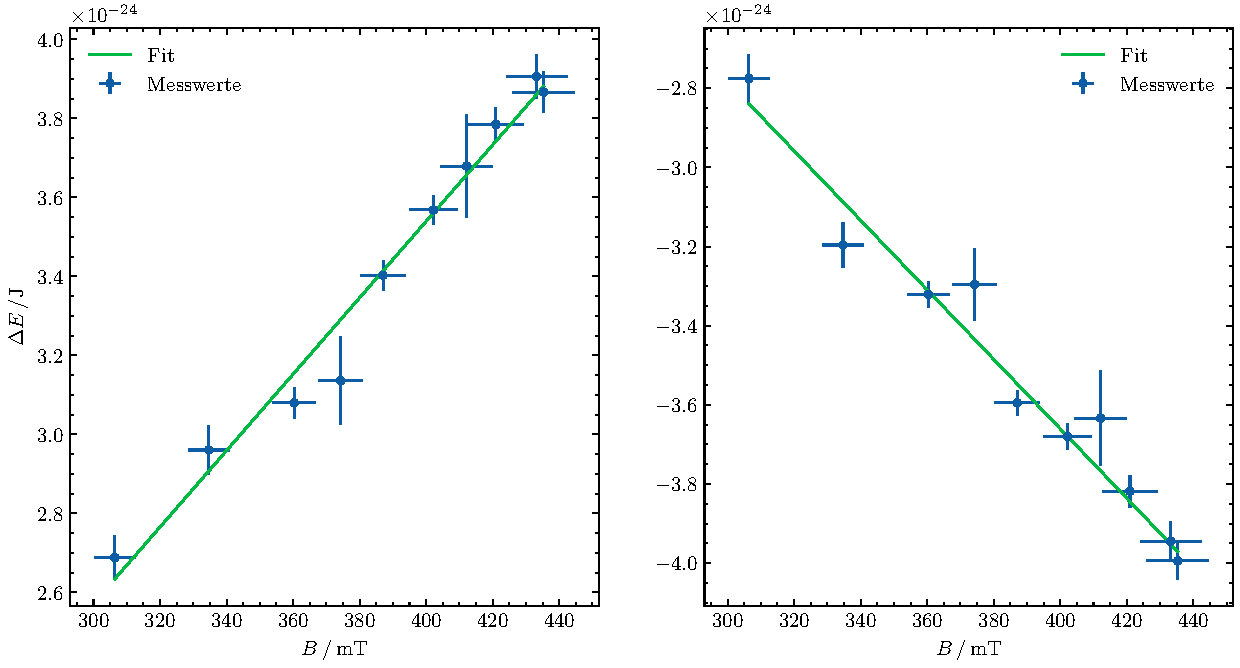
\includegraphics[width=0.9\linewidth]{../figs/magneton}
    \caption{Bestimmung des Bohrschen Magnetons}
    \label{fig:bohr_magneton}
\end{figure}

In \cref{fig:bohr_magneton} sind die Geradenanpassungen an die Magnetfeld-abhängige 
Energieverschiebung dargestellt. Da beide Geraden ein $\chi^2$ nahe 1 
besitzen, können diese als sehr gut betrachtet werden. Damit ergeben sich die Steigungen 
\begin{equation}
    \mu_\mathrm B^+ = \SI{9.7(5)e-24}{\joule\per\tesla}, 
    \qquad \mu_\mathrm B^- = \SI{8.8(6)e-24}{\joule\per\tesla}
    \label{eq:magneton_exp}.
\end{equation}
Verglichen mit dem Literaturwert $\mu_\mathrm B^\mathrm{Lit} = \SI{9.274}{\joule\per\tesla}$
liegt dieser in beiden Fällen im $1\sigma$-Bereich der Messung, wobei der relative 
Fehler bei etwa \qtyrange{5}{8}{\percent} liegt. Im Rahmen dieses Versuchs 
ist dies ein akzeptabler Wert. 

Weiterhin fällt auf, dass für $\sigma^\pm$-Strahlung der Wert jeweils über- oder unterschätzt 
wird. Wird aus beiden Messergebnissen der Mittelwert gebildet, so ergibt sich der 
Wert 
\begin{equation*}
    \mu_\mathrm B = \SI{9.3(8)e-24}{\joule\per\tesla},
\end{equation*}
was zwar eine höhere Unsicherheit besitzt, der Wert jedoch auf zwei signifikante Stellen 
genau dem Literaturwert entspricht. Es lässt sich somit vermuten, dass aufgrund 
von möglicher falscher Justierung das aufgenommene Bild verzerrt wurde und deshalb 
eine Abweichung nach oben und unten entsteht.

\subsection{weitere Überlegungen}
\subsubsection{Finesse und Auflösungsvermögen}
Die Finesse ist ein Maß für die Güte eines Resonators. Sie ist definiert als Quotient 
des freien Spektralbereiches und der Halbwertsbreite eines Maximums. 
\begin{equation}
    \mathcal F = \frac{\Delta\lambda}{\delta \lambda} = \frac{\pi\sqrt R}{1-R}.
    \label{fig:finesse}
\end{equation}
Mit dem bekannten Reflexionskoeffizienten $r=0.85$ des Etalons ergibt sich eine theoretische Finesse 
von 
\[\mathcal F_\mathrm{theo} = \num{19.3}.\]
Der freie Spektralbereich ist definiert als Frequenzunterschied zweier Beugungsordnungen. 
Mit \cref{eq:etalon_gleichung} ergibt sich somit 
\begin{equation*}
    \Delta\nu = \frac{c}{2d\sqrt{n^2-\sin^2\alpha}} \approx \frac{c}{2nd}
\end{equation*}
für kleine Winkel. In Ortsdarstellung lässt sich damit die Gleichung 
\begin{equation}
    \Delta\lambda = c\qty(\frac{1}{\nu_1} - \frac{1}{\nu_2})\approx \lambda^2\frac{\Delta\nu}{c}
        =  \frac{\lambda^2}{2nd}
    \label{fig:free_spectralrange}
\end{equation}
nähern. Das Auflösungsvermögen lässt sich mit \cref{fig:finesse,fig:free_spectralrange} 
für das Etalon daher mit
\begin{equation}
    A = \frac{\lambda}{\delta\lambda} = \frac{2nd}{\lambda}\mathcal F
    \label{eq:finesse}
\end{equation}
bestimmen. Für den genutzten Aufbau entspricht dies dem Auflösungsvermögen.
\[A_\mathrm{theo} = \num{3.5e5}\]
Das Auflösungsvermögen kann bestimmt werden, indem der Spulenstrom so lange 
verringert wird, bis die einzelnen Ringe durch den Zeeman-Effekt nicht mehr aufgelöst werden 
können. Mit \cref{eq:energieverschiebung} kann das Auflösungsvermögen als 
\[A = \frac{hc}{\lambda\mu B(I)}\]
geschrieben werden. Es wurden in transversaler und longitudinaler Richtung 
die Ströme 
\[I_\mathrm{transv} = \SI{3.6(1)}{\ampere},
\qquad I_\mathrm{longi} = \SI{1.3(2)}{\ampere}\]
gemessen. Da nach \cref{fig:bfield_kalibration} die Ströme sich im linearen Bereich 
der Kalibrationskurve befinden, kann die Unsicherheit mit 
$\Delta A = A\cdot\Delta I/I$
approximiert werden. Da in longitudinaler Richtung die mittlere Linie nicht sichtbar ist, muss 
in diesem Fall das Auflösungsvermögen zusätzlich um den Faktor 2 verringert werden.
Es ergeben sich die Werte 
\[A_\mathrm{transv} = \num{1.37(4)e5}, \qquad A_\mathrm{longi} = \num{1.9(3)e5},\]
womit der Referenzwert deutlich größer als die Messwerte sind. Dies könnte am wahrscheinlichsten 
an einer mangelnden Justierung liegen, in der die Sammellinse nicht vollständig fokussiert 
wurde. Dies würde auch die schlechte Auflösung der Zeeman-Aufspaltung in \cref{sec:magneton} 
erklären. Außerdem ist anzumerken, dass das Auflösungsvermögen in transversaler und longitudinaler Ausrichtung 
voneinander abweichen. Möglich ist ein einfacher 
Ablesefehler als Grund für die Abweichung, falls die Maxima als nicht unterscheidbar 
angesehen wurden, obwohl sie es eigentlich noch waren.
Die Finessen sind nach \cref{eq:finesse}
\[\mathcal F_\mathrm{trans} = \num{7.5\pm.3},\qquad \mathcal F_\mathrm{longi} = \num{10.4\pm1.7}.\]
Da diese linear mit dem Auflösungsvermögen zusammenhängen, sind diese auch nach unten 
verschoben.


\subsubsection{Dopplerverbreiterung}
Aufgrund der thermischen Bewegung der Atome in der Cadmiumlampe verschiebt sich 
nach dem Dopplereffekt die am Detektor gemessene Lichtwellenlänge. Bei Raumtemperatur
überwiegt dieser Effekt der natürlichen Linienbreite. Die Dopplerverbreiterung
ist mit der Gleichung 
\begin{equation*}
    \Delta\lambda = \frac{\lambda}{c}\sqrt{\frac{8k_\mathrm BT\ln 2}{m}}
\end{equation*}
berechenbar. Bei einer Temperatur von \SI{1000}{\kelvin} ergibt sich eine Verbreiterung von 
\SI{1.38}{\pm}.  Diese Breite wird mit der Linienbreite eines Maximums ohne Magnetfeld verglichen. 
Eine Gauß-Anpassung an das gleiche Maximum wie in \cref{sec:magneton} wurde in \cref{fig:doppler}
min einem linearen Offset vorgenommen. Es konnte aufgrund 
der Asymmetrie des Peaks keine Gauß-Funktion angepasst werden, die den gesamten Bereich des Maximums
gut beschreibt. Die Breite und der Mittelwert müssten trotzdem innerhalb der Unsicherheit 
gut abgeschätzt werden können. Diese sind $\alpha_0 = -\SI{.748(1)}{\degree}$ mit einer 
Standardabweichung $\sigma = \SI{0.041(1)}{\degree}$. Um daraus die Breite der Kurve 
in Ortsdarstellung zu bestimmten, wird zunächst \cref{eq:etalon_gleichung} für kleine Winkel genähert mit 
\begin{equation*}
    \lambda \approx \frac{2d}{m}\qty(n-\frac{\alpha^2}{2n}).
\end{equation*}
Mit der Definition $\Delta\alpha=\alpha_1 - \alpha_0$ lässt sich mit der Linienbreite folgendermaßen 
bestimmen:
\begin{align*}
    \Delta\lambda &= \lambda_1 - \lambda_0 = \frac{d}{mn}\qty(\alpha_0^2 - \alpha_1^2) 
    = \frac{d}{mn}(\alpha_0-\alpha_1)(\alpha_0 + \alpha_1)
    = -\frac{d}{mn}\Delta\alpha(\alpha_1 - \alpha_0 + 2\alpha_0)\\
    &= -\frac{d}{mn}\Delta\alpha(\Delta\alpha + 2\alpha_0).
\end{align*}
Die Dopplerverbreiterung bezieht sich jedoch auf die Halbwertsbreite, weshalb die Standardabweichung noch 
umgerechnet werden muss mit $\Delta\alpha = \sigma\sqrt{2\ln 2}$. Mit den Messwerten ergibt sich eine 
Verbreiterung von 
\begin{equation}
    \Delta\lambda_\mathrm{exp} = \SI{3.3(1)}{\pm}.
\end{equation}

Verglichen mit der Dopplerverbreiterung von etwa \SI{1.4}{\pm} liegt dieser Wert in derselben Größenordnung,
jedoch um über den Faktor 2 größer. Wird mit \cref{eq:finesse} das Auflösungsvermögen berechnet, 
so ergibt sich mit dem experimentellen Wert $A = \num{1.97(5)e5}$, was vergleichbar mit der Messung 
der longitudinalen Konfiguration ist. Es ist naheliegend, dass der Aufbau nicht richtig justiert wurde
und deshalb ein leicht unscharfes Bild bei der Messung entstanden ist, welche die Linienbreite erhöht.

\begin{figure}[h]
    \centering
    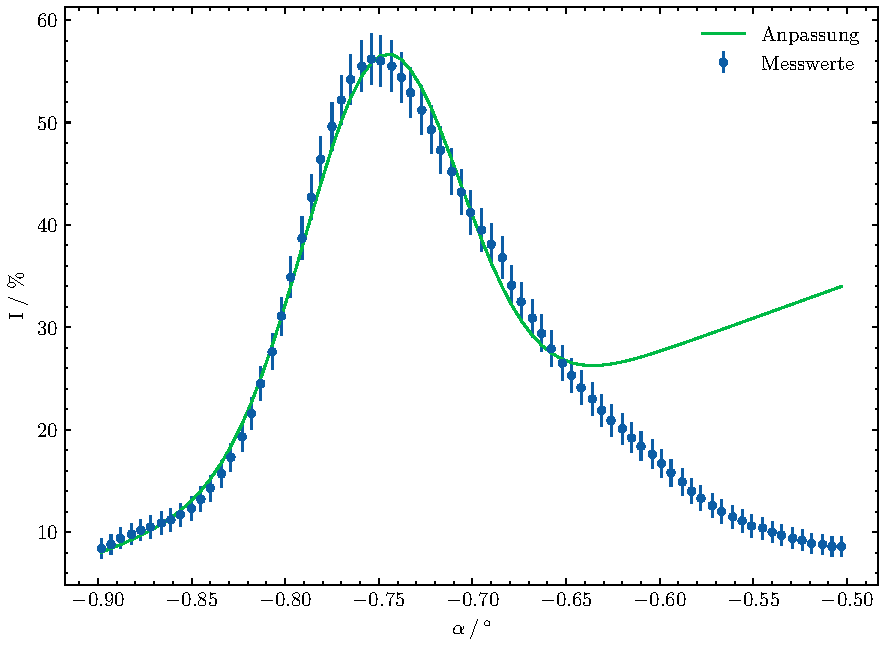
\includegraphics[width=0.5\linewidth]{../figs/doppler}
    \caption{Anpassung an ein Maximum bei Messung mit CCD-Kamera ohne angelegten Magnetfeld.}
    \label{fig:doppler}
\end{figure}

